\documentclass[conference]{IEEEtran}
\IEEEoverridecommandlockouts
% The preceding line is only needed to identify funding in the first footnote. If that is unneeded, please comment it out.
\usepackage{cite}
\usepackage{amsmath,amssymb,amsfonts}
\usepackage{algorithmic}
\usepackage{graphicx}
\usepackage{textcomp}
\usepackage{xcolor}
\usepackage{amsmath}
\def\BibTeX{{\rm B\kern-.05em{\sc i\kern-.025em b}\kern-.08em
    T\kern-.1667em\lower.7ex\hbox{E}\kern-.125emX}}
\begin{document}

\title{American sign language understanding\\}

\author{\IEEEauthorblockN{Duarte Mortágua}
\IEEEauthorblockA{\textit{DETI, UA} \\
\textit{Universidade de Aveiro}\\
Aveiro, Portugal \\
Número Mecanográfico: 92963}
\and
\IEEEauthorblockN{Mário Silva}
\IEEEauthorblockA{\textit{DETI, UA} \\
\textit{Universidade de Aveiro}\\
Aveiro, Portugal \\
Número Mecanográfico: 93430}
}

\maketitle

\begin{abstract}
Speech impairment is a disability that affects an individual’s ability to communicate using speech and hearing. People who have it, have to resort to another way of communication such as sign language. In recent times, there has been promising progress in the fields of gesture recognition and motion using deep learning and computer vision-based techniques, these technologies can help non-sign language speakers communicate with people with speech impairment. The database of hand gestures used for this paper represents a multi-class problem with 24 classes of letters (excluding J and Z which require motion).
\end{abstract}
\begin{IEEEkeywords}
Machine Learning, Sign Language Recognition, Classification, Deep Learning, Neural Networks
\end{IEEEkeywords}


\section{Introduction}
This report is made to demonstrate our apprenticeships and explain the reasons behind our decisions and thought process during the investigation phase of this project and throughout the course of TAA - Tópicos de Aprendizagem Automática.

The theme of our project is to design an algorithm that can understand and recognize the alphabet letters from hand gestures. Hand gestures and sign language are the most commonly used methods by deaf and non-speaking people to communicate among themselves or with speech-able people. People use sign language gestures as a means of non-verbal communication to express their thoughts and emotions. The National Institute on Deafness and Other Communications Disorders (NIDCD) indicates that the 200-year-old American Sign Language is a complete, complex language (of which letter gestures are only part) but is the primary language for many deaf North Americans. 


But non-signers find it extremely difficult to understand, hence trained sign language interpreters are needed during medical and legal appointments, educational, and training sessions, also, over the past five years, there has been an increasing demand for interpreting services. However, understanding sign language is not a universal skill. For this reason, building a system that recognizes hand gestures and sign language can be very useful to facilitate the communication gap between speech-able and speech impaired people.

A robust visual recognition algorithm, for example, one that uses modern machine learning methods such as Convolutional Neural Networks, could help the deaf and hard-of-hearing better communicate using computer vision applications.

\begin{figure}[htbp]
    \centerline{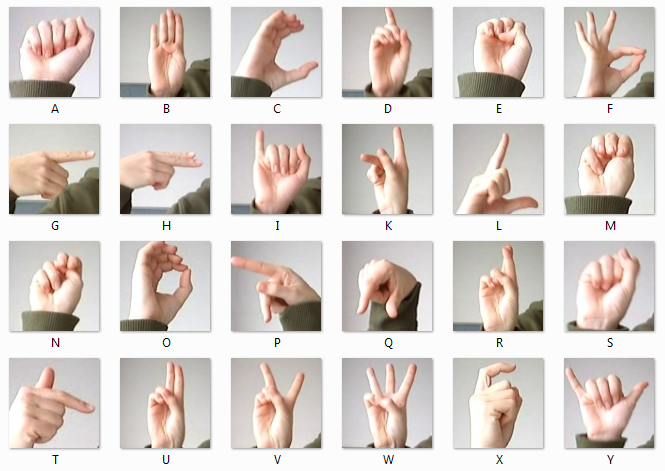
\includegraphics[width=8cm]{img/sign_language_example.png}}
    \caption{American Sign Language Letters}
    \label{fig:hist_train_classes}
\end{figure}


\section{Data-Set Analysis}

\subsection{Description}

The dataset used to feed our model is available here and provides 7172 images for testing and 27455 images for training. This images are labeled with a number in the range 0-25 as a one-to-one map for each alphabetic letter A-Z (and no cases for 9=J or 25=Z because of gesture motions). Each row represents an image, and each column represents one of the 784 pixels of the image (28x28 pixel image), being that each pixel has a color value of 0-255.

The Sign Language MNIST original data came from greatly extending the small number (1704) of the color images included as not cropped around the hand region of interest.\cite{kaggle} To create new data, an image pipeline was used by the authors of this dataset\cite{kaggle} and included cropping to hands-only, gray-scaling, resizing, and then creating at least 50+ variations to enlarge the quantity. The modification and expansion strategy was filters ('Mitchell', 'Robidoux', 'Catrom', 'Spline', 'Hermite'), along with 5\% random pixelation, +/- 15\% brightness/contrast, and finally 3 degrees rotation.

\subsection{Statistical Analysis}

As mentioned before, all the images in the dataset are labeled with one of 25 possible labels, each one representing one class in our model. We must notice that the distribution is not uniform, particularly in the test set. This would be a problem if the train set had the same kind of distribution, meaning that there would be classes with more or less images than others. Working with this biased data could lead to misjudging relatively to our model results, and could also be problematic when creating our Cross Validation subset more ahead.

\begin{figure}[htbp]
    \centerline{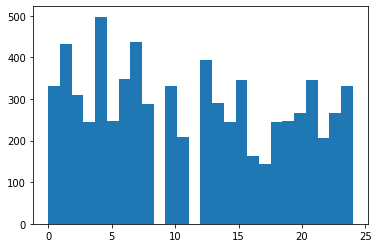
\includegraphics[width=8cm]{img/test_classes_hist.png}}
    \caption{Number of images per class in the Test Set}
    \label{fig:hist_test_classes}
\end{figure}
\begin{figure}[htbp]
    \centerline{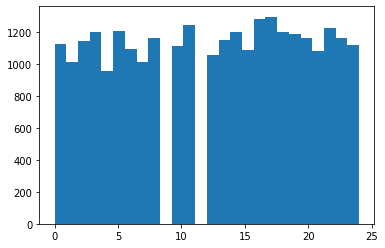
\includegraphics[width=8cm]{img/train_classes_hist.png}}
    \caption{Number of images per class in the Train Set}
    \label{fig:hist_train_classes}
\end{figure}

\section{Initial approach - Logistic Regression}
\subsection{Model description}
Logistic Regression is a type of analysis that is used if the goal is to determine the category/class of the output. It is a generalized linear model because the outcome always depends on the sum of the inputs and parameters. Or in other words, the output cannot depend on the product of its parameters.\cite{raschka}
In this case we’re taking a multi-class approximation of this type of analysis, since in this case logistic regression is used to determine the letter symbolized in the hand image, which may have 1 of 26 possible outcomes, and not just 2 (binary).
To achieve this, we’re using PyTorch’s built-in linear function, where each independent variable is multiplied by a weight and added by some offset bias affects the classification of the output.\cite{logistic-torch}
PyTorch’s linear function will output a tensor with 26 elements with each element denoting the probability that the image is that symbol.

\subsection{Loss Function and Optimizer}
To normalize the values returned by this function, PyTorch’s cross entropy function was used. This function combines the negative log likelihood and SoftMax function to normalize the resulting values from the linear function.\cite{logistic-torch}

\begin{equation}
\begin{split}
\operatorname{loss}(x, \text { class })=-\log \left(\frac{\exp (x[\text { class }])}{\sum_{j} \exp (x[j])}\right) \\
=-x[\text { class }]+\log \left(\sum_{j} \exp (x[j])\right)
\end{split}
\end{equation}

The optimizer will be the learning algorithm we use. In this case, we will use the Stochastic Gradient Descent.
\subsection{Initial hyperparameters}

In this model we have 3 hyperparameters, batch size, learning rate and epochs. The batch size dictates how many images the model will load at a time. The learning rate on the other hand dictates how large the model will adjust its parameters after every training phase. An epoch describes the number of times the algorithm sees the entire data set. So, each time the algorithm has seen all samples in the dataset, an epoch has completed. We decided the batch size and epochs based on the articles we have seen: batch size of 256 and 200 epochs.\cite{logistic-torch} To decide the learning rate, we tried with 8 different learning rates and observed the validation accuracy results as shown below:

\begin{figure}[htbp]
    \centerline{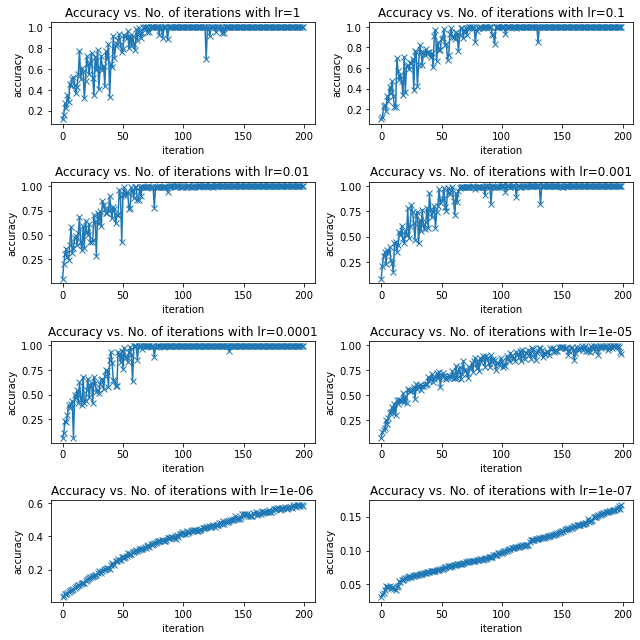
\includegraphics[width=9cm]{img/logisticRegression.png}}
    \caption{Accuracy per epoch validation during training with different learning rates}
    \label{fig:accuracy_per_epoch}
\end{figure}
\subsection{Results and change of approach}

As seen in all the graphs, as the number of epochs increases, the accuracy of the model increases. The most interesting learning rates are 0.01, where high accuracy is stable since 100 epochs but has an unstable growing with many accuracy dips, and 1e-05, where the stabilization is not completely achieved but the growing is more stable.
We decided to evaluate both models using the validation dataset and the testing dataset:

\begin{table}[htbp]
\caption{A. Accuracy and Loss on lr=1e-05 with 200 epochs}
\begin{center}
\begin{tabular}{|p{2cm}|p{2cm}|p{2cm}|}
\hline
\textbf{\textit{Set}}& \textbf{\textit{Loss}}& \textbf{\textit{Accuracy}} \\
\hline
Validation & 0.0703 & 0.9835 \\
\hline
Test & 5.5739 & 0.5628 \\
\hline
\end{tabular}
\end{center}
\end{table}

\begin{table}[htbp]
\caption{B.	Accuracy and Loss on lr=0.01 with 200 epochs}
\begin{center}
\begin{tabular}{|p{2cm}|p{2cm}|p{2cm}|}
\hline
\textbf{\textit{Set}}& \textbf{\textit{Loss}}& \textbf{\textit{Accuracy}} \\
\hline
Validation & 0.4703 & 0.9985 \\
\hline
Test & 1150.3939 & 0.6855 \\
\hline
\end{tabular}
\end{center}
\end{table}

In both cases we got good results on the accuracy of the validation set, as expected, but in the test set the results were not so good. Additionally, the loss in the second case was too high, making us only rely on model A.
To try getting better results in the model A, we trained this model for more 800 epochs, but it took no effect on the accuracy and loss results. \\

When we were searching about more ways to improve this model’s accuracy and reduce the loss, we concluded that a problem like this with multi class classification which involves image recognition is not going to get any better with a linear approach like the Logistic Regression. Instead, we decided to move to a Convolutional Neural Network model, since it successfully deals with complex images having pixel dependencies throughout. It also reduces the images into a form which is easier to process, without losing features which are critical for getting a good prediction.\cite{towardsdatascience_Saha}

\section{Convolutional Approach}

\subsection{The problem / approaches}

The advancements in Computer Vision with Deep Learning have been constructed and perfected with time, primarily over one particular algorithm — a Convolutional Neural Network. A Convolutional Neural Network (ConvNet/CNN) is a Deep Learning algorithm very used in the field of image recognition and classification.\cite{towardsdatascience_Saha}

\subsection{Architecture}

The main role of the ConvNet is to reduce the images into a form that is easier to process, without losing features that are critical for getting a good prediction. This is very important when the goal is to design an architecture that is not only good at learning features but also is scalable to bigger datasets. It can learn features and classify images that are much different from the ones given on the training data set and does this better than the logistic regression approach. Also, it performs a better fitting to the image dataset due to the reduction in the number of parameters involved and the re-usability of weights. In other words, the network can be trained to understand the sophistication of the image better.\cite{towardsdatascience_Saha}

\subsection{Base Arch Implementation}

1) \textit{Convolutional Layers} - The objective of a Convolution Layer is to extract the high-level features such as edges, from the input image. ConvNets need not be limited to only one Convolutional Layer. Conventionally, the first ConvLayer is responsible for capturing the Low-Level features such as edges, color, gradient orientation, etc. With added layers, the architecture adapts to the High-Level features as well, giving us a network which has the wholesome understanding of images in the dataset, similar to how we would.\cite{towardsdatascience_Saha} \\

2) \textit{Pooling Layer} - Similar to the Convolutional Layer, the Pooling layer is responsible for reducing the spatial size of the Convolved Feature. This is to decrease the computational power required to process the data through dimensionality reduction. Furthermore, it is useful for extracting dominant features which are rotational and positional invariant, thus maintaining the process of effectively training of the model. There are two types of Pooling: Max Pooling and Average Pooling. In this work we used Max Pooling, which also performs as a Noise Suppressant. It discards the noisy activations altogether and also performs de-noising along with dimensionality reduction.\cite{towardsdatascience_Saha} \\

The Convolutional Layer and the Pooling Layer, together form the i-th layer of a Convolutional Neural Network. Depending on the complexities in the images, the number of such layers may be increased for capturing low-levels details even further, but at the cost of more computational power.\cite{towardsdatascience_Saha} \\

3) \textit{Flattening Layer} - A flattening layer is a layer which aims to flattening the input, which means turning the complex matrix given into a vector. \\

4) \textit{Activation Layers} - They are responsible for transforming the summed weighted input from the node into the activation of the node or output for that input.
The rectified linear activation function or ReLU for short is a piece-wise linear function that will output the input directly if it is positive, otherwise, it will output zero. It has become the default activation function for many types of neural networks including CNN because a model that uses it is easier to train and often achieves better performance. Then, in order to classify our resulting features, we use Softmax Classification technique.\cite{towardsdatascience_Saha} \\

According to the above, our initial model implementation was the following:
\begin{figure}[htbp]
    \centerline{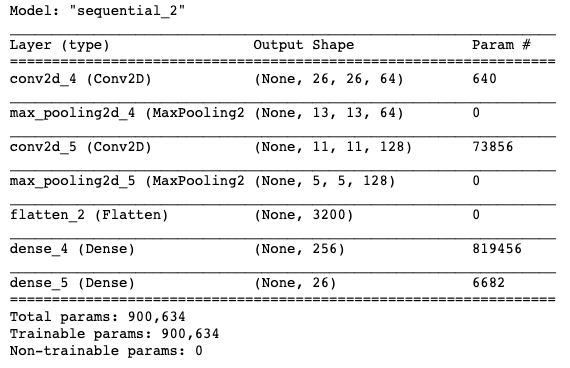
\includegraphics[width=9cm]{img/initial_model.png}}
    \caption{Initial CNN Model}
    \label{fig:hist_train_classes}
\end{figure}

The output layer of this model has 26 neurons for 26 different letters, and the activation function is softmax since it is a multiclass classification problem.

\section{Image Processing}

The Training Accuracy for the model used with CNN is 100\% while the test accuracy is 90\%. This represents a case where overfitting is happening and we will resort to some data augmentation techniques to attempt to fix this problem.

\begin{figure}[htbp]
    \centerline{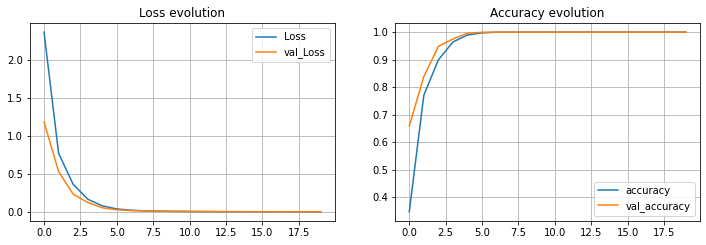
\includegraphics[width=9cm]{img/initial_model_noDataAug_20ep.png}}
    \caption{Initial CNN Model with 20 Epochs}
    \label{fig:hist_train_classes}
\end{figure}

\begin{table}[htbp]
\caption{Initial CNN Model with 20 Epochs}
\begin{center}
\begin{tabular}{|p{2cm}|p{2cm}|p{2cm}|}
\hline
\multicolumn{3}{|c|}{\textbf{Accuracies}} \\
\hline
\textbf{\textit{Test}}& \textbf{\textit{Validation}}& \textbf{\textit{Train}} \\
\hline
0.90685 & 0.99981 & 1.0 \\
\hline
\multicolumn{3}{|c|}{\textbf{Losses}} \\
\hline
\textbf{\textit{Test}}& \textbf{\textit{Validation}}& \textbf{\textit{Train}} \\
\hline
0.400423 & 0.00152 & 0.00105 \\
\hline
\end{tabular}
\end{center}
\end{table}

\subsection{Data Augmentation}

Sometimes there are more features in the test set than the ones present in the training one, therefore it doesn't have the highest accuracy it could have, one way of trying to increase it is by augmenting the data. This step is very important since it allows to keep high levels of accuracy even when the image to classify is different from the ones from the original dataset. It can be very useful for example in our case, a person can make hand signs with the right or left hand, therefore, we flip some of the images from the training set \cite{towardsdatascience_jachak}.

To augment data in the CNN model, we used TensorFlow's Image Data Generator method that allows us to do random alterations to the images, such as:

\begin{itemize}
\item Re-scales pixels of the image by dividing by 255.
\item Rotates images between 0 and 45 degrees.
\item Shifts images horizontally and vertically by 15\%.
\item Zooms in and out images by 20\%.
\item Flips images horizontally.
\end{itemize}

It also allows us to split the training data set into validation, for this we did some research and found that 20\% is usually a good percentage of validation data.

\section{MODEL AND HYPER-PARAMETER ALTERATIONS}

\subsection{Epochs}

With our initial model (Fig. 4) with just 20 epochs that took about 15 minutes to complete, it had a decent result, however, like said previously, it represented an overfitting scenario. To compete with this, we added data augmentation.

\begin{figure}[htbp]
    \centerline{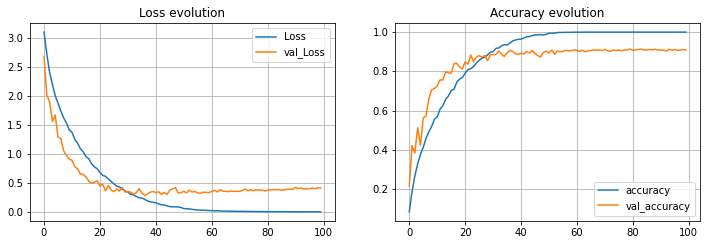
\includegraphics[width=9cm]{img/initial_model_100ep.png}}
    \caption{Initial CNN Model with Data Augmentation with 100 Epochs}
    \label{fig:hist_train_classes}
\end{figure}

\begin{table}[htbp]
\caption{Initial CNN Model with Data Augmentation with 100 Epochs}
\begin{center}
\begin{tabular}{|p{2cm}|p{2cm}|p{2cm}|}
\hline
\multicolumn{3}{|c|}{\textbf{Accuracies}} \\
\hline
\textbf{\textit{Test}}& \textbf{\textit{Validation}}& \textbf{\textit{Train}} \\
\hline
0.87632 & 0.90857 & 1.0 \\
\hline
\multicolumn{3}{|c|}{\textbf{Losses}} \\
\hline
\textbf{\textit{Test}}& \textbf{\textit{Validation}}& \textbf{\textit{Train}} \\
\hline
0.57181 & 0.41203 & 0.002130 \\
\hline
\end{tabular}
\end{center}
\end{table}

With these results (Table IV), we see a decrease in test accuracy in comparison to the previous trainning, but it makes sence since we added data augmentation to the training data set. Looking at the graphic (Fig. 7) we can see the validation accuracy couldn't go higher than 90\%, one of the reasons for this is because the validation set does not have the data augmented and therefore we concluded that the data augmentation was a bit too much, some images changed a lot that started being recognized as others, so we also decided to tweak the values a little lower after this to try and reach a more balanced prediction.

Also, we believe this in fact resolved the overfitting problem as the next training sessions the values of test accuracy and training accuracy were not as far apart as the initial model without data augmentation.

Running 100 epochs took a little over an hour to complete, in contrast to the previous which only took 15 minutes. In relation to the number of epochs, after interpreting the graphic (Fig. 7), we realized the values stagnated at around 50 epochs, so from here we decided to run only 50 epochs which took half the time and had similar values.

\subsection{Changes in the Neural Network Structure}

\subsubsection{Batch Normalization}

Batch normalization is a layer that allows every layer of the network to do learning more independently. It is used to normalize the output of the previous layers. The activations scale the input layer in normalization. Using batch normalization learning becomes efficient also it can be used as regularization to avoid overfitting of the model. The layer is added to the sequential model to standardize the input or the outputs \cite{towardsdatascience_jachak}. 

After running 100 epochs, we realized it took way too much time to get good accuracy, with an average of 35 seconds per epoch it took over an hour as said previously. So, we started looking at other ways of improving the time and found Batch Normalisation.

This layer allows normalizing the inputs of the hidden layer. Just like we did before and normalized the input layer, for example, by rescaling the image’s pixel value between o to 1, in a similar fashion, Batch Normalization normalizes the input provided to the hidden layers. As from the above model, we can see that though, with data augmentation, we resolved overfitting the training data but it required a lot more time. There are several advantages of Batch Normalisation but the most promising ones are requiring less number of epochs, learning of hidden layer is more independent of each other, and has less covariance shift, that is it prevents the model from overfitting.

\begin{figure}[htbp]
    \centerline{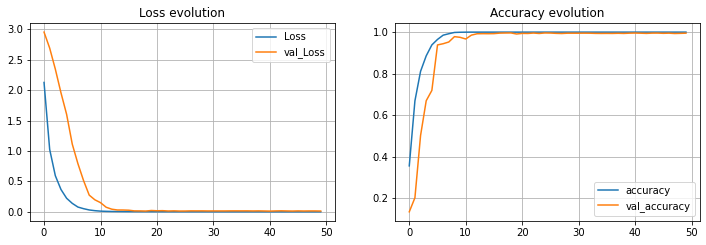
\includegraphics[width=9cm]{img/final_model_batch_50ep.png}}
    \caption{CNN Model with Data Augmentation and Batch Normalization layers with 50 Epochs}
    \label{fig:hist_train_classes}
\end{figure}

\begin{table}[htbp]
\caption{Accuracies and Losses of CNN Model with Data Augmentation and Batch Normalization layers with 50 Epochs}
\begin{center}
\begin{tabular}{|p{2cm}|p{2cm}|p{2cm}|}
\hline
\multicolumn{3}{|c|}{\textbf{Accuracies}} \\
\hline
\textbf{\textit{Test}}& \textbf{\textit{Validation}}& \textbf{\textit{Train}} \\
\hline
0.97921 & 0.98140 & 1.0 \\
\hline
\multicolumn{3}{|c|}{\textbf{Losses}} \\
\hline
\textbf{\textit{Test}}& \textbf{\textit{Validation}}& \textbf{\textit{Train}} \\
\hline
0.05824 & 0.06313 & 0.38846 \\
\hline
\end{tabular}
\end{center}
\end{table}


The Training accuracy after including batch normalization is 100\% and test accuracy is 98\%. And by analysing the graph, the validation accuracy stagnates at just 15 epochs, that is less than half of the epochs without batch normalization. And also it after the first iterations the time decreased each time and the average time per iteration was of 15 seconds which is less than half of the model without Batch Normalization.

\subsubsection{Dropout}

During the training phase of the neural network, some nodes in a hidden layer are dropped randomly based on their neuron value. This allows the network to be architecturally different at each run and hence, preventing overfitting \cite{medium_Jachak}. We started with a dropout rate of 0.4 and experimented a bit to find a sweet spot. We got good results at a rate of 0.3.

\begin{figure}[htbp]
    \centerline{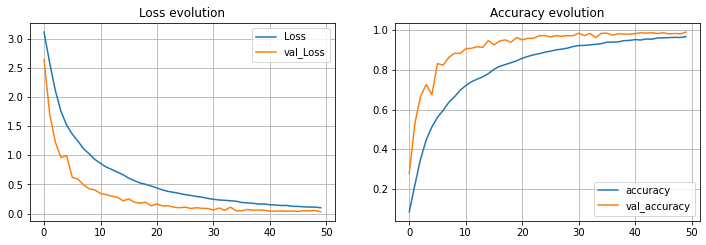
\includegraphics[width=9cm]{img/final_model_drop_50ep.png}}
    \caption{CNN Model with Data Augmentation and Dropout layers with 50 Epochs}
    \label{fig:hist_train_classes}
\end{figure}

\begin{table}[htbp]
\caption{CNN Model with Data Augmentation and Dropout layers with 50 Epochs}
\begin{center}
\begin{tabular}{|p{2cm}|p{2cm}|p{2cm}|}
\hline
\multicolumn{3}{|c|}{\textbf{Accuracies}} \\
\hline
\textbf{\textit{Test}}& \textbf{\textit{Validation}}& \textbf{\textit{Train}} \\
\hline
0.97755 & 0.99125 & 0.99776 \\
\hline
\multicolumn{3}{|c|}{\textbf{Losses}} \\
\hline
\textbf{\textit{Test}}& \textbf{\textit{Validation}}& \textbf{\textit{Train}} \\
\hline
0.06593 & 0.03168 & 0.03138 \\
\hline
\end{tabular}
\end{center}
\end{table}


As we can see from the graph (Fig. 7), between the iterations 0 and 30 there are a significantly increases and decreases in the validation losses, comparing to this model, there are a bit less bumps and the line is smoother. However accuracies were a little bit surprising to us at first, since the training accuracy was lower than the validation accuracy.

This seemed counter intuitive, since usually training accuracy is higher or same as the validation. As mentioned before one reason is because we only use data augmentation on the training set, the images from the validation set are easier to predict the correct labels, but after doing some research we found out that the main reason for this is because the dropout regularization layer is only activated when training but deactivated when evaluating on the validation.


\subsection{Decaying Learning Rate}

Since the validation accuracies weren't fluctuating a lot and the lines were fairly smooth we didn't implement decaying learning rate, however it is worth mentioning. If the learning rate was too high it could cause the model to overshoot the optima and a great way of avoiding that would be the use of a decaying learning rate which drops the learning rate by some value after each epoch \cite{towardsdatascience_jachak}.

\subsection{Batch Size}

Batch size is one of the most important hyperparameters to tune in modern deep learning systems. Practitioners often want to use a larger batch size to train their model as it allows computational speedups from the parallelism of GPUs. However, it is well known that too large of a batch size will lead to poor generalization \cite{medium_Shen}.

Using smaller batch sizes have been empirically shown to have faster convergence to “good” solutions. This is intuitively explained by the fact that smaller batch sizes allow the model to “start learning before having to see all the data.” The downside of using a smaller batch size is that the model is not guaranteed to converge to the global optima. 

Since we had a few computational constraints we started off with a bigger batch size of 512 and also because we found on an article \cite{analytics} that it was a good value for this problem. Then we got curious and tested with other batch sizes as well.

\begin{table}[htbp]
\caption{Test Accuracies of the CNN Model with Different Batch Sizes}
\begin{center}
\begin{tabular}{|p{2cm}|p{2cm}|}
\hline
\textbf{\textit{Batch Sizes}} & \textbf{\textit{Test Accuracies}} \\
\hline
\textbf{32} & 91\% \\
\hline
\textbf{64} & 95\% \\
\hline
\textbf{128} & 93\% \\
\hline
\textbf{256} & 92\% \\
\hline
\textbf{512} & 98\% \\
\hline
\textbf{1024} & 93\% \\
\hline
\end{tabular}
\end{center}
\end{table}

Looking at the results (Table VII) a batch size of 256 was indeed the best size for our case.

\subsection{Final CNN Model}

At the end, we merged the two previous models with Batch Normalization and Dropout layers (Fig. 11) and ended up with the best results.

Dropouts are usually advised not to use after the convolution layers, they are mostly used after the dense layers of the network, so we decided to put it there. Batch Normalization layers can be used at several points in between the layers of the model and is often placed just after defining the sequential model and after the convolution and pooling layers, for us, what showed the best results were just one layer and right after the convolutional layer.

Looking at the table (Table VIII), we concluded we have a model with a good fit – Validation accuracy high, slightly lower than the training accuracy.

\begin{figure}[htbp]
    \centerline{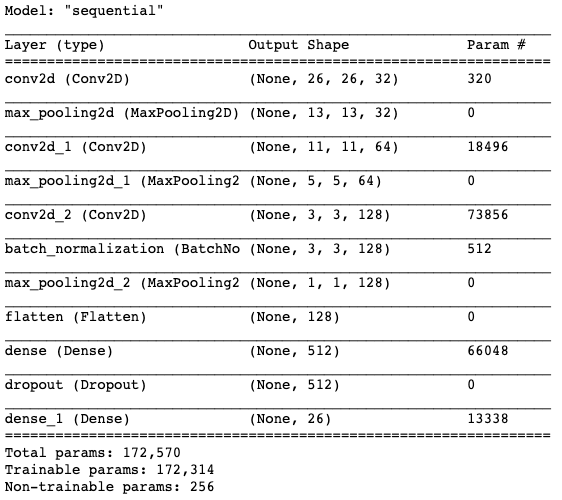
\includegraphics[width=9cm]{img/final_model_summary.png}}
    \caption{Final CNN Model Summary}
    \label{fig:hist_train_classes}
\end{figure}

\begin{figure}[htbp]
    \centerline{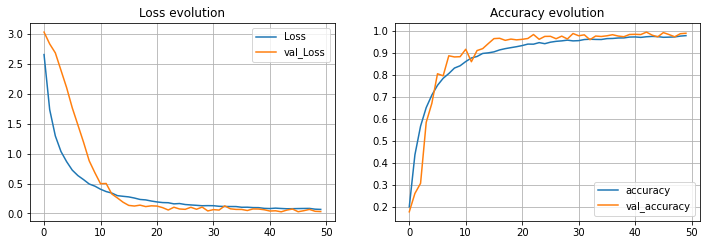
\includegraphics[width=9cm]{img/final_model_50ep.png}}
    \caption{Final CNN Model with 50 Epochs}
    \label{fig:hist_train_classes}
\end{figure}

\begin{table}[htbp]
\caption{Accuracies and Losses of Final CNN Model with 50 Epochs}
\begin{center}
\begin{tabular}{|p{2cm}|p{2cm}|p{2cm}|}
\hline
\multicolumn{3}{|c|}{\textbf{Accuracies}} \\
\hline
\textbf{\textit{Test}}& \textbf{\textit{Validation}}& \textbf{\textit{Train}} \\
\hline
0.98728 & 0.99501 & 0.99604 \\
\hline
\multicolumn{3}{|c|}{\textbf{Losses}} \\
\hline
\textbf{\textit{Test Loss}}& \textbf{\textit{Validation Loss}}& \textbf{\textit{Train Loss}} \\
\hline
0.05589 & 0.03144 & 0.01971 \\
\hline
\end{tabular}
\end{center}
\end{table}

We also ran our final model against the data without augmenting it (Fig. 12), the results are as we expected since it still happens the same overfitting problem as it did before, even though the results were still pretty good with 93\% accuracy (Table VIII) for the test data, and it had that result with just 14 epochs haven taken only 3 minutes to complete the training.

\begin{figure}[htbp]
    \centerline{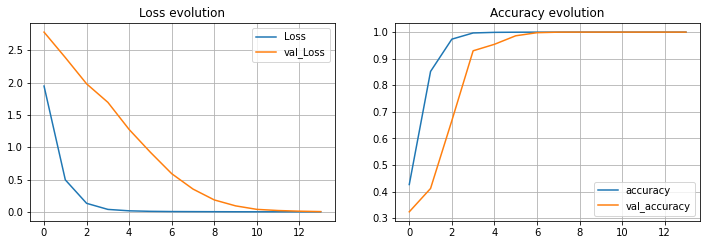
\includegraphics[width=9cm]{img/final_model_noDataAug.png}}
    \caption{Final CNN Model without Data Augmentation with 14 Epochs}
    \label{fig:hist_train_classes}
\end{figure}

\begin{table}[htbp]
\caption{Accuracies and Losses of Final CNN Model without Data Augmentation with 14 Epochs}
\begin{center}
\begin{tabular}{|p{2cm}|p{2cm}|p{2cm}|}
\hline
\multicolumn{3}{|c|}{\textbf{Accuracies}} \\
\hline
\textbf{\textit{Test}}& \textbf{\textit{Validation}}& \textbf{\textit{Train}} \\
\hline
0.93307 & 1.0 & 1.0 \\
\hline
\multicolumn{3}{|c|}{\textbf{Losses}} \\
\hline
\textbf{\textit{Test Loss}}& \textbf{\textit{Validation Loss}}& \textbf{\textit{Train Loss}} \\
\hline
0.23590 & 0.00442 & 0.00390 \\
\hline
\end{tabular}
\end{center}
\end{table}


To summarize and visualize the performance of the CNN classification predictions we also made a confusion matrix. This helps us understand where the model was most confused and what type of errors it had. By analysing the normalized and non-normalized confusion matrixes (Fig. 13 and Fig. 14) we noticed it had mistaken a few letters for others that are actually very similar.

\begin{figure}[htbp]
    \centerline{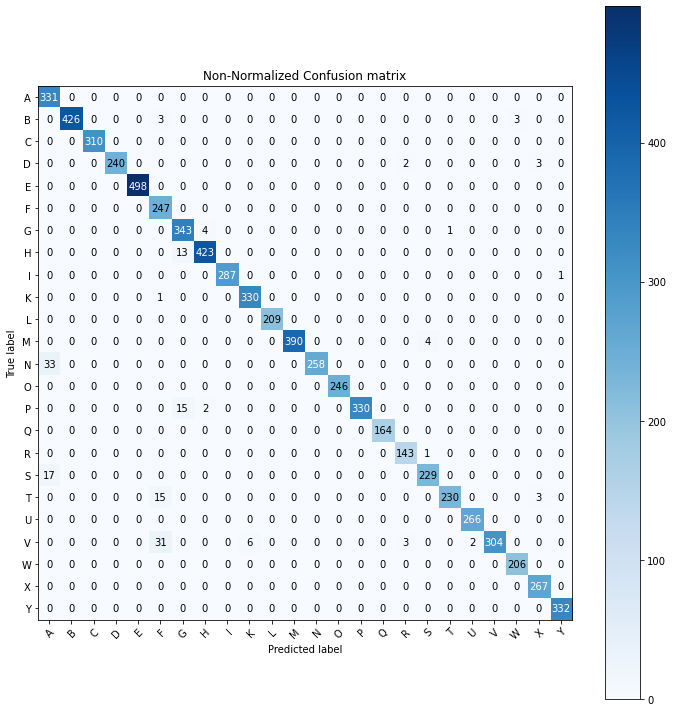
\includegraphics[width=9cm,height=8cm]{img/non_normalized_confusion_matrix.png}}
    \caption{Final CNN Model Normalized Confusion Matrix}
    \label{fig:hist_train_classes}
\end{figure}


\begin{figure}[htbp]
    \centerline{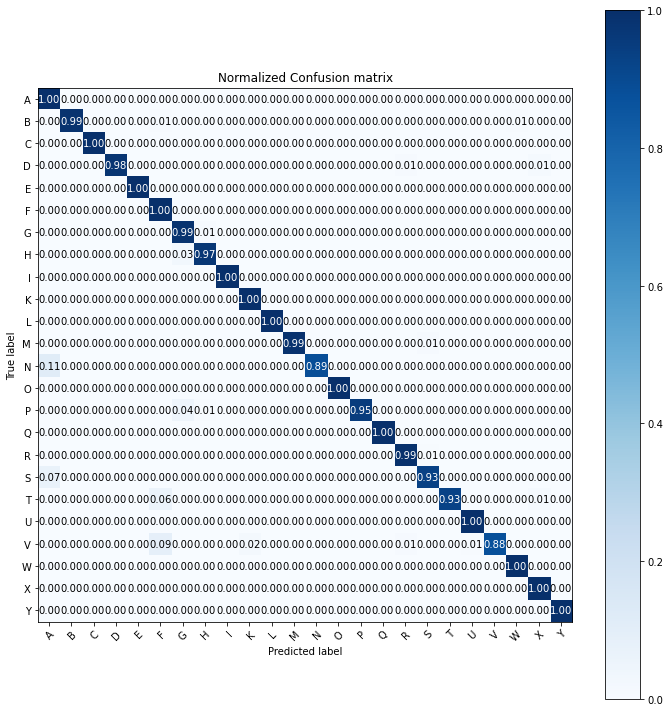
\includegraphics[width=9cm,height=8cm]{img/normalized_confusion_matrix.png}}
    \caption{Final CNN Model Non-Normalized Confusion Matrix}
    \label{fig:hist_train_classes}
\end{figure}

By looking at the final CNN model predicted classes (Fig. 15) we can visualize the mistake the model did, on the third row and fourth column, the model predicted an A letter while in fact it was an S. This proves exactly what the confusion matrix shows us, having 229 predictions on letter S correct and mistaken 17 of those for the letter A, and also for the letter N out of 291 it mistaken 33 times for the letter A. This makes us wonder why the letter A was always the prevailing one, since it had 100\% accuracy on it. We think it might be because the distributions of letters wasn't  equal and also because the model gave more weight to the features from the letter A than with S and N.

\begin{figure}[htbp]
    \centerline{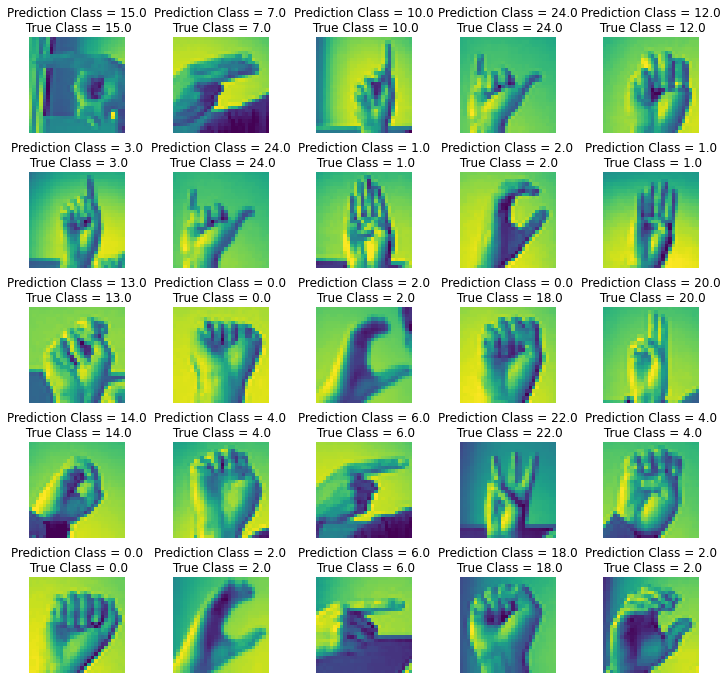
\includegraphics[width=9cm,height=8cm]{img/final_model_predictions.png}}
    \caption{Final CNN Model Predicted Classes}
    \label{fig:hist_train_classes}
\end{figure}


Also, by looking at the Figure 16 with the representation of the letter's A, N and S in hand gestures, we can understand how the model can make mistake on these because they are in fact very similar and even for a non trained person it would be hard to differentiate.

\begin{figure}[htbp]
    \centerline{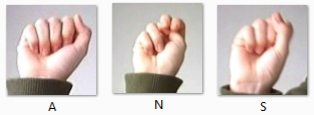
\includegraphics[width=6cm,height=2cm]{img/letters_comparison.png}}
    \caption{Letter's A, N and S comparison.}
    \label{fig:hist_train_classes}
\end{figure}


\section{Conclusions and how to improve}

The Logistic Regression model doesn't work so well when it comes to classifying images based on a wide range of inputs (non-binary).
In cases of extremely basic binary images, the method might show an average precision score while performing prediction of classes but would would not perform so well when it comes to more complex images having pixel dependencies throughout.\cite{towardsdatascience_Saha}

Images of the data set are very similar, they are all centered, no rotations, and had same distance of the hand to the camera.

We decided to test the models and took a few pictures of hand gestures with a phone, then did the necessary processing of the images, such as resizing them to 28x28 pixels, converted to a similar color scale as the initial data set and then divided the pixels by 255. After that we calculated the predictions with both models.

The CNN model had an accuracy of 83\% getting the right label class on 5 out of 6 images. Also, the only picture it failed to correctly predict was really similar to the one it actually is, it predicted the letter N instead of the letter A. We expected somewhat close results since we believe our model works well with images that aren't exactly equal, pixel by pixel, to the ones from the initial data set, since we did data augmentation and also a CNN model is already good for extracting features from images, therefore, they work better with other images which may have some differences.

\begin{figure}[htbp]
    \centerline{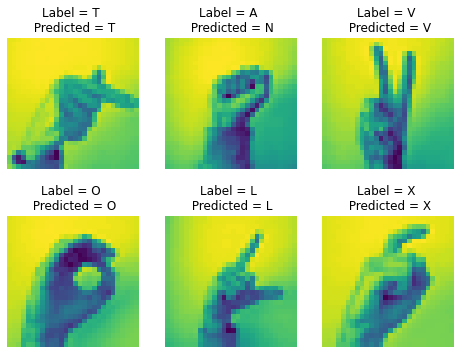
\includegraphics[width=6cm,height=5cm]{img/cnn_prediction_test.png}}
    \caption{Final CNN Model Predicted Classes}
    \label{fig:hist_train_classes}
\end{figure}

Also, by looking at Figure 16 with the representation of the letters A, N and S in hand gestures, we can understand how the model can make mistakes on these because they are very similar, even for a non trained person it would be hard to differentiate.

\begin{figure}[htbp]
    \centerline{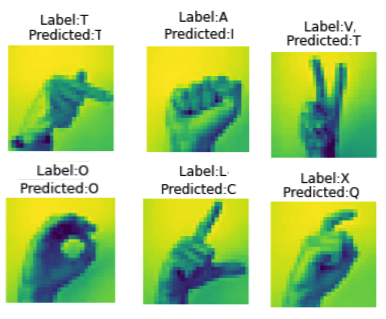
\includegraphics[width=6cm,height=5cm]{img/logistic_prediction_custom_data.png}}
    \caption{Logistic Regression Predicted Classes}
    \label{fig:logistic_predict_custom}
\end{figure}

Using K fold cross validation could lead to more accurate results, but since our data set is big enough we didn't found necessary as it would cost a lot of computation power.\cite{cross-val}

\begin{thebibliography}{00}

\bibitem{kaggle} Sign Language MNIST. (2017, October 20). Kaggle. https://www.kaggle.com/datamunge/sign-language-mnist/
\bibitem{raschka} Why is logistic regression considered a linear model? (2021, April 26). Dr. Sebastian Raschka.
bhttps://sebastianraschka.com/faq/docs/logistic\_regression\_linear.html
\bibitem{logistic-torch} Galario, G. (2020, June 29). Image Classification using Logistic Regression on the American Sign Language MNIST. Medium. https://medium.com/@gryangalario/image-classification-using-logistic-regression-on-the-american-sign-language-mnist-9c6522242ddf
\bibitem{medium_Jachak} Jachak, R. (2020, April 4). Getting it to top 6\% in Kaggle’s MNIST Digit Recognizer from scratch -3. Medium. https://medium.com/analytics-vidhya/getting-it-to-top-6-in-kaggles-mnist-digit-recognizer-from-scratch-3-8b11b79958a2
\bibitem{towardsdatascience_jachak} Jachak, R. (2020b, May 2). American Sign Language Recognition - Towards Data Science. Medium. https://towardsdatascience.com/american-sign-language-recognition-using-cnn-36910b86d651
\bibitem{towardsdatascience_Saha} Saha, S. (2020, October 15). A Comprehensive Guide to Convolutional Neural Networks — the ELI5 way. Medium. https://towardsdatascience.com/a-comprehensive-guide-to-convolutional-neural-networks-the-eli5-way-3bd2b1164a53
\bibitem{analytics} Kumar, V. (2020, October 25). Hands-On Guide To Sign Language Classification Using CNN. Analytics India Magazine. https://analyticsindiamag.com/hands-on-guide-to-sign-language-classification-using-cnn/
\bibitem{medium_Shen} Shen, K. (2018, June 20). Effect of batch size on training dynamics - Mini Distill. Medium. https://medium.com/mini-distill/effect-of-batch-size-on-training-dynamics-21c14f7a716e
\bibitem{kaggle_rushike} R. (2020, April 22). MNIST Sign Language Recognition CNN 99.94\%accuracy. Kaggle. https://www.kaggle.com/rushikesh0203/mnist-sign-language-recognition-cnn-99-94-accuracy
\bibitem{kaggle_sandee} S. (2021, April 24). Sign Language Identifier (100\% Accuracy TF Model). Kaggle. https://www.kaggle.com/sandeepbhogaraju/sign-language-identifier-100-accuracy-tf-model
\bibitem{cross-val} Arif, A. (2020, December 27). Cross Validation In Machine Learning. Dataaspirant. https://dataaspirant.com/cross-validation/
\end{thebibliography}


\end{document}
